\section{مبانی آماری و کران‌های اطلاعاتی}
\label{sec:bg:statistical-foundations}

در بخش \ref{sec:bg:f-divergence}، ابزارهای سنجش فاصله بین توزیع‌ها (خانواده $f$-واگرایی‌ها) را معرفی کردیم. در این بخش، قصد داریم با ایجاد پلی میان این مفاهیم انتزاعی و مسأله‌ی عملیاتی «تخمین پارامتر»، زیربنای ریاضی لازم برای تحلیل عملکرد تخمین‌گرها را بنا کنیم. تعاریف و لم‌های ارائه شده در ادامه، ابزارهای اصلی ما برای اثبات کران‌های پایین مینی‌مکس در فصل‌های آتی خواهند بود.

 \subsection{نظریه تصمیم و ریسک مینی‌مکس}
\label{sec:bg:minimax-risk}

در چارچوب «نظریه تصمیم آماری»\LTRfootnote{Statistical Decision Theory}، مسئله‌ی تخمین را می‌توان به عنوان یک بازی بین «طبیعت» (که پارامتر $\thh$ را انتخاب می‌کند) و «آمارگر» (که تخمین‌گر $\hat{\thh}$ را انتخاب می‌کند) مدل‌سازی کرد.

فرض کنید فضای نمونه $\Xset^n$ و کلاس مدل‌های آماری $\mathcal{P} = \{P_\thh : \thh \in \Thh\}$ داده شده‌اند. داده‌های مشاهده‌شده $X^n = (X_1, \dots, X_n)$ متغیرهای تصادفی مستقلی هستند که از توزیع $P_\thh$ تولید شده‌اند. برای سنجش کیفیت یک تخمین‌گر $\hat{\thh}$، به یک معیار فاصله‌ی متریک (یا شبه‌متریک) $\rho: \Thh \times \Thh \to \mathbb{R}_{\ge 0}$ روی فضای پارامتر نیاز داریم.

\begin{تعریف}[تابع زیان\LTRfootnote{Loss Function}]
میزان جریمه‌ی ناشی از تخمین پارامتر $\thh$ با مقدار $\hat{\thh}$، توسط تابع زیان اندازه‌گیری می‌شود که معمولاً تابعی صعودی از فاصله متریک است:
\begin{equation}
L\left(\hat{\thh}(X^n), \thh\right) \triangleq \Phi\left( \rho\left(\hat{\thh}(X^n), \thh\right) \right),
\end{equation}
که در آن $\Phi: [0, \infty) \to [0, \infty)$ تابعی غیرنزولی با شرط $\Phi(0)=0$ است. انتخاب‌های رایج شامل $\Phi(t)=t^2$ (زیان مربعات) و $\Phi(t)=|t|$ (زیان قدرمطلق) است.
\end{تعریف}

از آن‌جا که مشاهدات $X^n$ تصادفی هستند، مقدار زیان نیز یک متغیر تصادفی است. برای حذف تصادف، از امیدریاضی زیان استفاده می‌کنیم.

\begin{تعریف}[ریسک نقطه‌ای\LTRfootnote{Pointwise Risk}]
ریسک یک تخمین‌گر ثابت $\hat{\thh}$ در نقطه پارامتری مشخص $\thh$، برابر است با میانگین زیان وارده تحت توزیع $P_\thh$:
\begin{equation}
R(\hat{\thh}, \thh) \triangleq \Eset_{X^n \sim P_\thh^n} \left[ L\left(\hat{\thh}(X^n), \thh\right) \right].
\end{equation}
\end{تعریف}

از آن‌جا که پارامتر واقعی $\thh$ ناشناخته است، نمی‌توان تخمین‌گری یافت که ریسک نقطه‌ای آن برای تمام مقادیر $\thh$ کمینه باشد. برای حل این مشکل، رویکرد «مینی‌مکس»\LTRfootnote{Minimax Approach} بدترین حالت ممکن را در نظر می‌گیرد.

\begin{تعریف}[ریسک مینی‌مکس]
\label{def:minimax-rate}
ریسک مینی‌مکس برای کلاس $\mathcal{P}$ و متریک $\rho$، برابر است با کم‌ترین مقدارِ بیشینه‌ریسک ممکن بر روی تمامی تخمین‌گرهای اندازه‌پذیر. به بیان دقیق ریاضی:
\begin{equation}
\label{eq:minimax-def}
\begin{split}
\mathfrak{M}_n(\Thh, \Phi \circ \rho) 
&\triangleq \inf_{\hat{\thh}} \sup_{\thh \in \Thh} R(\hat{\thh}, \thh) \\
&= \inf_{\hat{\thh}} \sup_{\thh \in \Thh} \Eset_{X^n \sim P_\thh^n} \left[ \Phi\left(\rho\left(\hat{\thh}(X^n), \thh\right)\right) \right].
\end{split}
\end{equation}
هدف اصلی نظریه مینی‌مکس، یافتن کران‌های پایین و بالا برای این کمیت بر حسب اندازه نمونه $n$ است.
\end{تعریف}

\subsection{تقلیل به آزمون فرض (روش بسته‌بندی)}
\label{sec:bg:hypothesis-testing}

محاسبه مستقیم مقدار \eqref{eq:minimax-def} دشوار است. استراتژی استاندارد ما برای غلبه بر این دشواری، «تبدیل فضای پیوسته پارامتر به یک مجموعه گسسته» است. به عبارت دیگر، مسئله‌ی «تخمین» را به مسئله‌ی «آزمون فرض چندگزینه‌ای» تقلیل می‌دهیم.

این فرآیند بر پایه این شهود استوار است که هر تخمین‌گر دقیق، باید بتواند بین پارامترهایی که فاصله‌ی تقریباً زیادی از هم دارند، تمایز قائل شود. برای رسمی‌سازی این ایده، از مفهوم «بسته‌بندی» استفاده می‌کنیم.

\begin{تعریف}[مجموعه بسته‌بندی]
مجموعه‌ی متناهی $\mathcal{V} = \{\thh_1, \dots, \thh_M\} \subset \Thh$ یک $2\delta$-بسته‌بندی\LTRfootnote{Packing} برای فضای $(\Thh, \rho)$ نامیده می‌شود اگر اعضای آن حداقل به اندازه $2\delta$ از یک‌دیگر فاصله داشته باشند:
\begin{equation}
\min_{i \neq j} \rho\left(\thh_i, \thh_j\right) \ge 2\delta
\label{eq:deltapackineq}
\end{equation}
\end{تعریف}
\begin{figure}[ht]
    \centering
    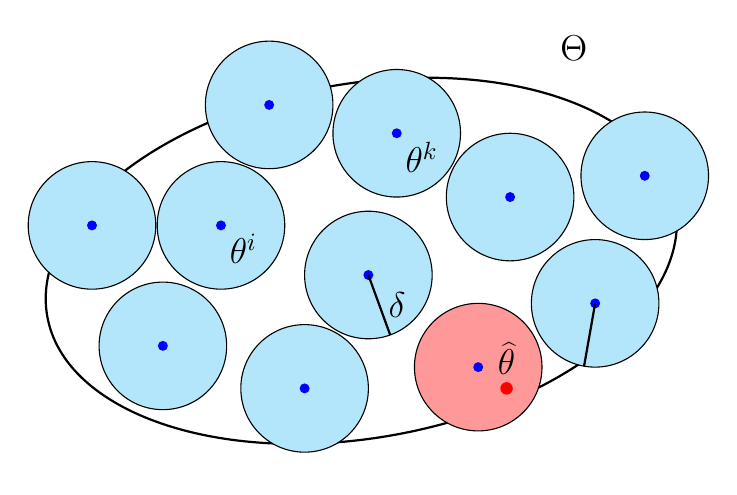
\begin{tikzpicture}[scale=0.9, every node/.style={transform shape}]
        % تنظیمات اولیه
        \def\R{0.9} % شعاع دایره‌های کوچک

        % 1. رسم بیضی بزرگ (فضای پارامتر تتا)
        \draw[thick, rotate=10] (0,0) ellipse (4.5cm and 2.5cm);
        \node at (3, 3) {\Large $\Theta$};

        % 2. دایره‌های آبی (بسته‌بندی)
        \tikzstyle{packball} = [circle, draw=black, fill=cyan!30, minimum size=2*\R cm, inner sep=0pt]
        
        % دایره بالا (theta^k)
        \node[packball] (c1) at (0.5, 1.8) {};
        \fill[blue] (c1.center) circle (2pt) node[below right, black] {\Large $\theta^k$};

        % دایره چپ (theta^i)
        \node[packball] (c2) at (-1.98, .5) {};
        \fill[blue] (c2.center) circle (2pt) node[below right, black] {\Large $\theta^i$};
        
        % دایره‌های دیگر (تزئینی برای نشان دادن پر شدن فضا)
        \node[packball] at (-1.3, 2.2) {};
        \fill[blue] (-1.3, 2.2) circle (2pt);
        
        \node[packball] at (-3.8, .5) {}; 
        \fill[blue] (-3.8, .5) circle (2pt);
        
        \node[packball] at (-2.8, -1.2) {}; 
        \fill[blue] (-2.8, -1.2) circle (2pt);

        \node[packball] at (-0.8, -1.8) {}; 
        \fill[blue] (-0.8, -1.8) circle (2pt);

        \node[packball] at (2.1, .9) {}; 
        \fill[blue] (2.1, .9) circle (2pt);
        
        \node[packball] at (4, 1.2) {}; 
        \fill[blue] (4, 1.2) circle (2pt);

        % دایره مرکزی (نشان‌دهنده شعاع دلتا)
        \node[packball] (c_center) at (0.1, -0.2) {};
        \fill[blue] (c_center.center) circle (2pt);
        % رسم خط شعاع
        \draw[thick] (c_center.center) -- node[right] {\Large $\delta$} ++(-70:\R);

        % دایره راست (با خط شعاع)
        \node[packball] (c_right) at (3.3, -0.6) {};
        \fill[blue] (c_right.center) circle (2pt);
        \draw[thick] (c_right.center) -- ++(-100:\R);

        % 3. دایره قرمز (ناحیه تخمین‌گر)
        \node[circle, draw=black, fill=red!40, minimum size=2*\R cm, inner sep=0pt] (c_red) at (1.65, -1.5) {};
        % مرکز دایره (پارامتر واقعی)
        \fill[blue] (c_red.center) circle (2pt);
        % نقطه تخمین‌گر (قرمز)
        \fill[red] (c_red.center) ++(0.4, -0.3) circle (2.5pt) node[above=2pt, black] {\Large $\widehat{\theta}$};

    \end{tikzpicture}
    \caption{\rl{نمایش هندسی روش بسته‌بندی برای تقلیل مسئله‌ی تخمین به آزمون فرض. فضای پارامتر $\Theta$ با مجموعه‌ای از گوی‌های مجزا $\{\theta^1, \dots, \theta^K\}$ پوشانده شده است که تشکیل یک $2\delta$-بسته‌بندی می‌دهند. اگر تخمین‌گر $\widehat{\theta}$ (نقطه قرمز) دارای خطای کم‌تر از $\delta$ باشد، لزوماً درون یکی از این گوی‌ها قرار می‌گیرد. از آن‌جا که گوی‌ها مجزا هستند، حداکثر یک اندیس $i$ وجود دارد که $\widehat{\theta}$ به آن نزدیک باشد؛ لذا مسئله تخمین به یافتن این اندیس (آزمون فرض چندگزینه‌ای) تقلیل می‌یابد.}}
    \label{fig:packing-fano}
\end{figure}

می‌توانیم قضیه‌ی زیر را که به صورت عمومی برای کران پایین ریسک مینی‌مکس ثابت کنیم:
\begin{قضیه}[کران پایین عمومی]
فرض کنید $\{\thh_1, \dots, \thh_M\}$ یک $2\delta$-بسته‌بندی برای $\Thh$ باشد. آن‌گاه ریسک مینی‌مکس به خطای آزمون فرض محدود می‌شود:
\begin{align}
\mathfrak{M}_n(\Thh) &\ge \Phi(\delta) \cdot \inf_{\hat{\thh}} \sup_{\thh \in \mathcal{V}} \Pr_{P_\thh^n}\left(\rho\left(\hat{\thh}, \thh\right) \ge \delta\right) \\
&\ge \Phi(\delta) \cdot \inf_{\psi} \bar{P}_{err}(\psi) \label{eq:reduction-inequality}
\end{align}
که در آن $\bar{P}_{err}(\psi) = \frac{1}{M} \sum_{v=1}^M P_{\thh_v}^n\left(\psi(X^n) \neq v\right)$ میانگین احتمال خطا روی فرضیه‌های گسسته است و $\psi$ آزمون‌گری است که سعی در بازیافت اندیس $v$ دارد.
\end{قضیه}

\begin{اثبات}
برای اثبات این قضیه، از تعریف ریسک مینی‌مکس و خواص مجموعه‌های بسته‌بندی استفاده می‌کنیم. روند اثبات طی چند مرحله‌ی منطقی به شرح زیر انجام می‌شود:

\textbf{۱. محدود کردن فضای پارامتر:}
طبق تعریف ریسک مینی‌مکس (رابطه \ref{eq:minimax-def})، ماکزیمم ریسک روی تمام فضای $\Thh$ محاسبه می‌شود. از آن‌جا که مجموعه‌ی بسته‌بندی $\mathcal{V} = \{\thh_1, \dots, \thh_M\}$ زیرمجموعه‌ای از $\Thh$ است ($\mathcal{V} \subset \Thh$)، سوپریمم روی $\Thh$ همواره بزرگ‌تر یا مساوی سوپریمم روی $\mathcal{V}$ خواهد بود. هم‌چنین، ماکزیمم خطا همواره از میانگین خطا بزرگ‌تر است. بنابراین داریم:
\begin{align}
\mathfrak{M}_n(\Thh) &= \inf_{\hat{\thh}} \sup_{\thh \in \Thh} \Eset_{P_\thh} \left[ \Phi(\rho(\hat{\thh}, \thh)) \right] \nonumber \\
&\ge \inf_{\hat{\thh}} \sup_{\thh \in \mathcal{V}} \Eset_{P_\thh} \left[ \Phi(\rho(\hat{\thh}, \thh)) \right] \nonumber \\
&\ge \inf_{\hat{\thh}} \frac{1}{M} \sum_{v=1}^M \Eset_{P_{\thh_v}} \left[ \Phi(\rho(\hat{\thh}, \thh_v)) \right] \label{eq:proof-step1}
\end{align}

\textbf{۲. استفاده از نامساوی مارکوف:}
از آن‌جا که $\Phi$ تابعی صعودی و غیرمنفی است، می‌توانیم از نامساوی مارکوف استفاده کنیم. برای هر $\thh$ ثابت داریم:
\begin{align}
\Eset \left[ \Phi(\rho(\hat{\thh}, \thh)) \right] &\ge \Eset \left[ \Phi(\rho(\hat{\thh}, \thh)) \cdot \mathbb{I}(\rho(\hat{\thh}, \thh) \ge \delta) \right] \nonumber \\
&\ge \Phi(\delta) \cdot \Pr \left( \rho(\hat{\thh}, \thh) \ge \delta \right) \label{eq:proof-step2}
\end{align}

\textbf{۳. ساخت آزمون‌گر از روی تخمین‌گر:}
فرض کنید متغیر تصادفی $V$ به صورت یکنواخت از بین اندیس‌های $\{1, \dots, M\}$ انتخاب شود. برای هر تخمین‌گر دل‌خواه $\hat{\thh}$، می‌توانیم یک آزمون‌گر (تست) $\psi: \mathcal{X}^n \to \{1, \dots, M\}$ بر اساس قاعده‌ی «کم‌ترین فاصله» بسازیم:
\begin{equation}
\psi(X^n) = \arg \min_{k \in \{1, \dots, M\}} \rho(\hat{\thh}(X^n), \thh_k)
\end{equation}

\textbf{۴. تحلیل خطا با نامساوی مثلث:}
نکته‌ی کلیدی این است که نشان دهیم اگر تخمین‌گر $\hat{\thh}$ به پارامتر واقعی نزدیک باشد، آزمون‌گر لزوماً اندیس درست را باز می‌گرداند.
فرض کنید اندیس واقعی $v$ باشد. اگر آزمون‌گر دچار خطا شود (یعنی $\psi(X^n) \neq v$)، به این معنی است که یک اندیس $k \neq v$ وجود دارد که تخمین‌گر به $\thh_k$ نزدیک‌تر (یا مساوی) است تا به $\thh_v$:
\begin{equation}
\rho(\hat{\thh}, \thh_k) \le \rho(\hat{\thh}, \thh_v)
\end{equation}
از طرفی، چون $\mathcal{V}$ یک $2\delta$-بسته‌بندی است، طبق نامساوی مثلث داریم:
\begin{align}
2\delta &\le \rho(\thh_v, \thh_k) \quad \text{(تعریف بسته‌بندی)} \nonumber \\
&\le \rho(\thh_v, \hat{\thh}) + \rho(\hat{\thh}, \thh_k) \quad \text{(نامساوی مثلث)} \nonumber \\
&\le \rho(\thh_v, \hat{\thh}) + \rho(\hat{\thh}, \thh_v) \quad \text{(شرط خطای آزمون)} \nonumber \\
&= 2\rho(\hat{\thh}, \thh_v)
\end{align}
نتیجه می‌گیریم که وقوع خطای آزمون ($\psi \neq v$) مستلزم وقوع خطای تخمین بزرگ ($\rho \ge \delta$) است:
\begin{equation}
\{\psi(X^n) \neq v\} \subseteq \{\rho(\hat{\thh}, \thh_v) \ge \delta\}
\end{equation}
و در نتیجه برای احتمالات داریم:
\begin{equation}
\Pr_{P_{\thh_v}} (\psi(X^n) \neq v) \le \Pr_{P_{\thh_v}} (\rho(\hat{\thh}, \thh_v) \ge \delta)
\label{eq:proof-step4}
\end{equation}

\textbf{۵. جمع‌بندی:}
با جایگذاری \ref{eq:proof-step4} در نامساوی مارکوف (\ref{eq:proof-step2}) و میانگین‌گیری روی تمام $v$ها (مرحله ۱)، داریم:
\begin{align}
\mathfrak{M}_n(\Thh) &\ge \frac{1}{M} \sum_{v=1}^M \Phi(\delta) \cdot \Pr(\rho(\hat{\thh}, \thh_v) \ge \delta) \nonumber \\
&\ge \Phi(\delta) \cdot \frac{1}{M} \sum_{v=1}^M \Pr(\psi(X^n) \neq v) \nonumber \\
&= \Phi(\delta) \cdot \bar{P}_{err}(\psi)
\end{align}
چون این رابطه برای هر تخمین‌گر $\hat{\thh}$ (و آزمون‌گر متناظر $\psi$) برقرار است، پس برای اینفیمم آن‌ها نیز صادق است.
\end{اثبات}

\subsection{نامساوی‌های کران پایین}
\label{sec:bg:lower-bounds}

اکنون که مسئله را به آزمون فرض روی $M$ نقطه تقلیل دادیم، برای اثبات کران‌های پایین نهایی نیاز به ابزارهایی داریم که $\bar{P}_{err}$ را از پایین محدود کنند. سه روش اصلی که بر پایه $f$-واگرایی‌ها بنا شده‌اند عبارتند از:

\begin{قضیه}[نامساوی لو کم\LTRfootnote{Le Cam's Inequality}]
\label{thm:le-cam}
این روش معمولاً برای آزمون بین دو توزیع $P_1$ و $P_2$ ($M=2$) استفاده می‌شود و برای «کران‌های محلی» حول یک نقطه مناسب است.
\begin{equation}
\label{eq:le-cam}
\inf_{\psi} \bar{P}_{err}(\psi) \ge \frac{1}{2} \left( 1 - \left\|P_1^n - P_2^n\right\|_{TV} \right)
\end{equation}
\textbf{تفسیر:} این نامساوی بیان می‌کند که اگر فاصله $TV$ بین دو توزیع کم باشد، همپوشانی آن‌ها زیاد است و هیچ آزمون‌گری نمی‌تواند با خطای ناچیز آن‌ها را تفکیک کند.
\end{قضیه}

\begin{قضیه}[نامساوی فانو\LTRfootnote{Fano's Inequality}]
\label{thm:fano}
زمانی که پارامتر مورد نظر متعلق به مجموعه‌ای بزرگ‌تر $\mathcal{V}$ باشد \\ ($M = |V| > 2$)، نامساوی فانو کران پایین قوی‌تری ارائه می‌دهد:
\begin{equation}
\label{eq:fano}
\inf_{\psi} \bar{P}_{err}(\psi) \ge 1 - \frac{I\left(X^n; V\right) + \log 2}{\log M}
\end{equation}
که در آن $I(X^n; V)$ اطلاعات متقابل بین داده‌ها و اندیس پارامتر است.

\textbf{تفسیر:} نامساوی فانو مسئله خطا را به اطلاعات متقابل $I(X^n; V)$ گره می‌زند. اگر داده‌ها حاوی اطلاعات کافی درباره اندیس واقعی $V$ نباشند (ظرفیت کانال نسبت به تعداد فرضیه‌ها $\log M$ کم باشد)، خطا اجتناب‌ناپذیر است.
\end{قضیه}

\begin{لم}[لم اسود\LTRfootnote{Assouad's Lemma}]
\label{lem:assouad}
این لم ابزاری قدرتمند برای فضاهای پارامتر با ابعاد بالا (مانند $\{-1, 1\}^d$) است. قدرت لم اسود در شکستن یک مسئله $d$-بعدی دشوار به $d$ مسئله ۱-بعدی مستقل است.
\begin{equation}
\label{eq:assouad}
\mathfrak{M}_n(\Thh) \ge \frac{\delta}{2} \sum_{j=1}^d \left[ 1 - \left\|M_{+j}^n - M_{-j}^n\right\|_{TV} \right]
\end{equation}
که در آن $M_{+j}^n$ و $M_{-j}^n$ توزیع‌های مخلوط حاشیه‌ای هستند (میانگین توزیع‌هایی که بیت $j$-ام آن‌ها به ترتیب $+1$ و $-1$ است). اگر در هر بُعد تمایز قائل شدن سخت باشد، مجموع خطاها با تعداد ابعاد $d$ جمع شده و کران دقیقی\LTRfootnote{Tight Bound} می‌سازد.
\end{لم}